\documentclass[10pt]{beamer}

\usetheme[progressbar=frametitle]{metropolis}
\usepackage{appendixnumberbeamer}

\usepackage{booktabs}
\usepackage[scale=2]{ccicons}

\usepackage{pgfplots}
\usepgfplotslibrary{dateplot}

\usepackage{xspace}
\newcommand{\themename}{\textbf{\textsc{metropolis}}\xspace}


% ---
% PACOTES
% --
\usepackage[alf]{abntex2cite}		% Citações padrão ABNT
\usepackage[brazil]{babel}		    % Idioma do documento
\usepackage{color}			       % Controle das cores
\usepackage[T1]{fontenc}		  % Selecao de codigos de fonte.
\usepackage{graphicx}			    % Inclusão de gráficos
\usepackage[utf8]{inputenc}		   % Codificacao do documento (conversão automática dos acentos)
\usepackage{multirow}
\usepackage{threeparttable}
\usepackage[capposition=top]{floatrow}
\usepackage{txfonts}			 % Fontes virtuais
\usepackage{ragged2e}
\usepackage{etoolbox}
\usepackage{lipsum}
\usepackage{amssymb}
% ---

% ---
% Minhas Definições
% ---

%Deixando o Caption alinhado a esquerda mesmo com quebra de linha
\usepackage[labelfont=bf, justification=justified,singlelinecheck=true]{caption}

%Justificando o corpo do texto
\renewcommand{\raggedright}{\leftskip=0pt \rightskip=0pt plus 0cm} 

% Colocando numero de paginas no slide
\setbeamertemplate{footline}[frame number]{}
\setbeamertemplate{caption}[numbered]{}




\title{AskMath}
\subtitle{Um Ambiente Virtual de Aprendizagem para Auxiliar no Processo de Ensino e Aprendizagem de Matem\'atica}
\date{\today}
% \date{}
\author{Marciano Saraiva e Samy Soares}
\institute{Universidade Federal do Cear\'a - Campus de Quixad\'a}
\titlegraphic{\hfill
\includegraphics[height=1.5cm]{figuras/logo.pdf}}

\begin{document}

\maketitle

\begin{frame}{Roteiro}
  \setbeamertemplate{section in toc}[sections numbered]
  \tableofcontents[hideallsubsections]
\end{frame}

\section{Introdu\c{c}\~ao}

%% ----------------- NOVO SLIDE --------------------------------
\begin{frame}{Sobre}

\begin{figure}[H]
  \centering
   \begin{minipage}[b]{0.25\textwidth}\end{minipage}
  \hfill
  \begin{minipage}[b]{0.3\textwidth}
	
\includegraphics[width=\textwidth]{figuras/askmath.png}
  \end{minipage}
  \hfill
  \begin{minipage}[b]{0.1\textwidth}
    
\includegraphics[width=\textwidth]{figuras/vs.png}
  \end{minipage}
  \hfill
  \begin{minipage}[b]{0.3\textwidth}
    
\includegraphics[width=\textwidth]{figuras/petti.png}
  \end{minipage}
  \hfill
  \begin{minipage}[b]{0.25\textwidth}\end{minipage}
\end{figure}

O AskMath é uma iniciativa do grupo PET–Tecnologia da Informação e objetiva prover uma plataforma de ensino para auxiliar estudantes do 
ensino médio e superior em seu processo de aprendizagem de Matemática.

\end{frame}

%% ----------------- NOVO SLIDE --------------------------------
\begin{frame}{Motivação}

\begin{itemize}
	\item Grande número de reprovações e desistências em turmas iniciais de Matemática de cursos na Universidade Federal do Ceará - Campus 
Quixadá.
	\item A Organização para Cooperação e Desenvolvimento Econômico(OECD) revelou que em 2015, 67.1\% do alunos brasileiros estavam abaixo 
do nível 2 (os níveis vão de 1 a 6) de proficiência em matemática na escala do PISA \cite{pisainfocus2016}.
\end{itemize}

\end{frame}

\section{P\'ublico-alvo}
%% ----------------- NOVO SLIDE --------------------------------
\begin{frame}{Público-alvo}

\begin{itemize}
	\item \textbf{Estudantes do ensino médio} que buscam uma ferramenta para praticar o conhecimento adquirido nas aulas
	\item \textbf{Ingressantes no ensino superior} que possuem deficiências de matemática em sua formação desde o ensino m\'edio
	\item \textbf{Professores de Matemática} que desejam acompanhar o andamento de sua turma
\end{itemize}

\end{frame}

\section{O Ambiente}

%% ----------------- NOVO SLIDE --------------------------------
\begin{frame}{Li\c{c}\~oes Fragmentadas}
	\begin{figure}[H]
		\centering
		\caption{Representa\c{c}\~ao da Hierarquia entre li\c{c}\~oes}
		 \begin{minipage}[b]{0.6\textwidth}
			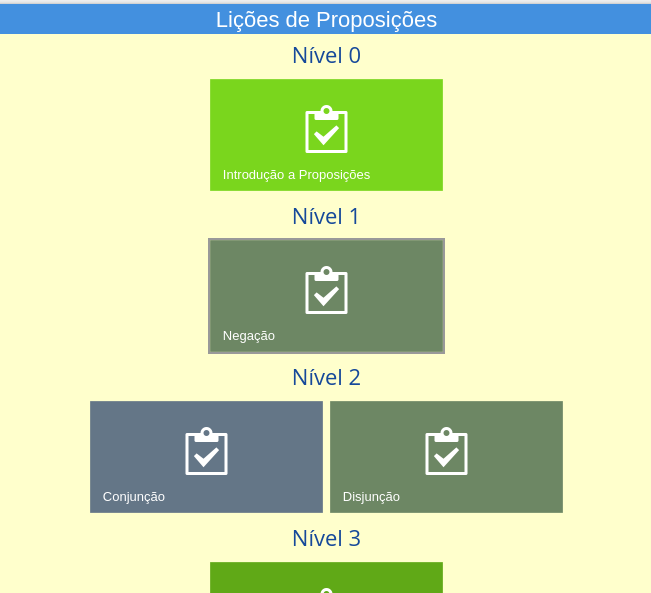
\includegraphics[width=\textwidth]{figuras/licoes.png}
		\end{minipage}
		\floatfoot{Fonte: <www.askmath.quixada.ufc.br>}
	\end{figure}
\end{frame}

%% ----------------- NOVO SLIDE --------------------------------
\begin{frame}{Resolu\c{c}\~ao de Problemas}
	\begin{figure}[H]
		\centering
		 \caption{Exemplo de um Problema}
		 \begin{minipage}[b]{1\textwidth}
			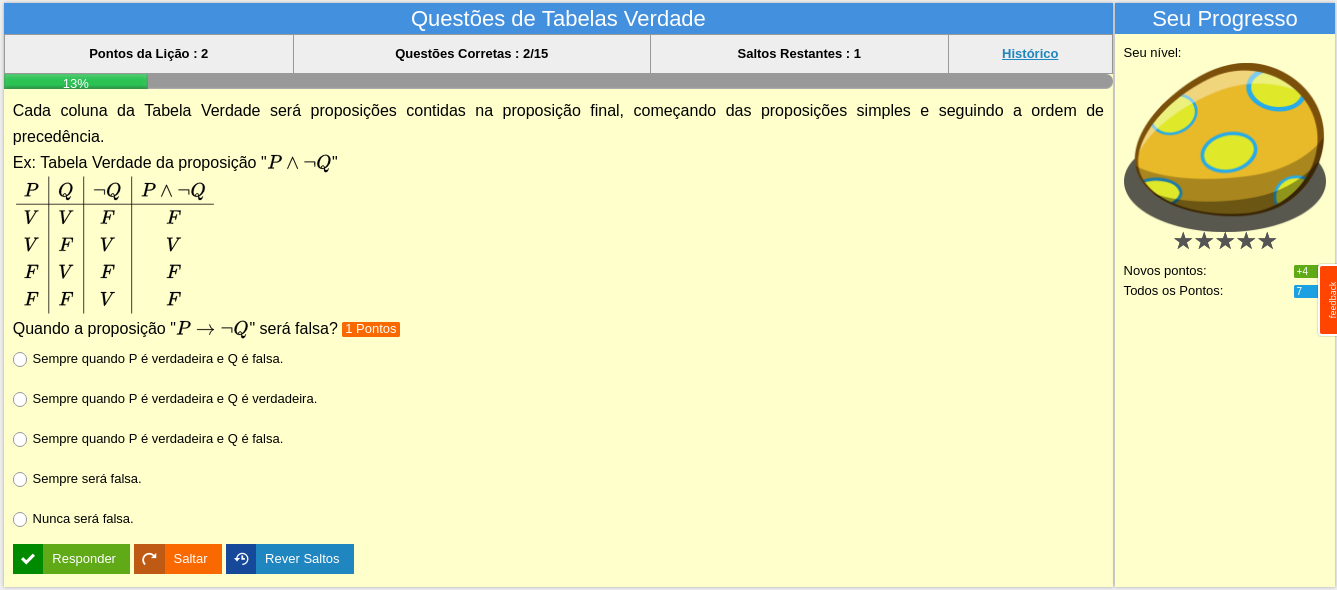
\includegraphics[width=\textwidth]{figuras/resolucao_problemas.png}
		\end{minipage}
		\floatfoot{Fonte: <www.askmath.quixada.ufc.br>}
	\end{figure}
\end{frame}

%% ----------------- NOVO SLIDE --------------------------------
\begin{frame}{Fórum de Discussões}
	\begin{figure}[H]
		\centering
		\caption{F\'orum de Discussões}
		 \begin{minipage}[b]{1\textwidth}
			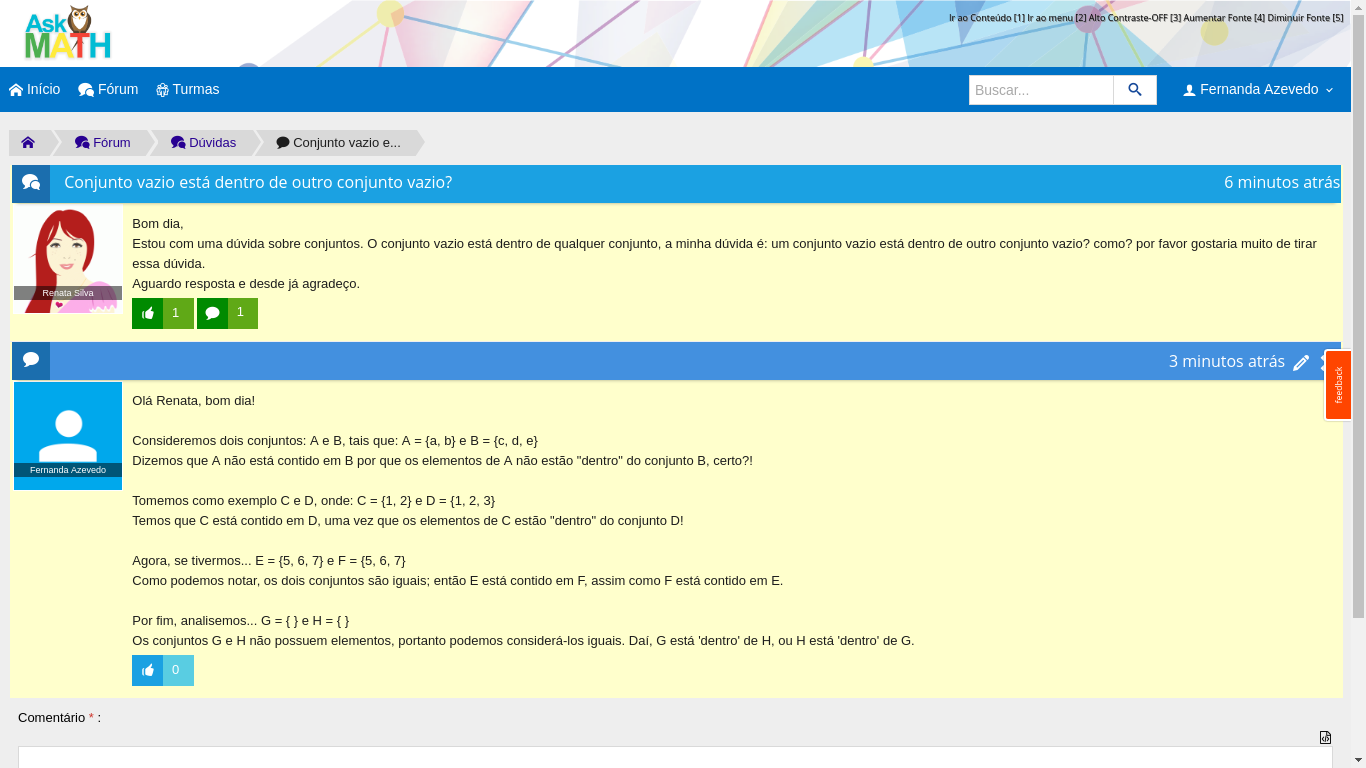
\includegraphics[width=\textwidth]{figuras/forum.png}
		\end{minipage}
		\floatfoot{Fonte: <www.askmath.quixada.ufc.br>}
	\end{figure}
\end{frame}

\section{Diferencial}

% ----------------- NOVO SLIDE --------------------------------


\begin{frame}{Identifica\c{c}\~ao das deficiências no Aprendizado}

\begin{overprint}
\only<+>{
	\begin{figure}[H]
	\centering
	\caption{Representa\c{c}\~ao do nosso Modelo de Aprendizagem}
	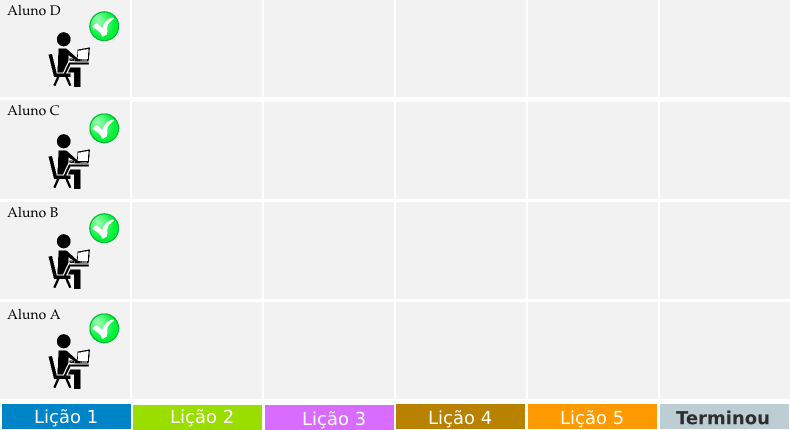
\includegraphics[width=8cm]{figuras/proposta/imagem1.png}
	\floatfoot{Fonte: Elaborada pelo autor}
	\end{figure}
}
\only<+>{
	\begin{figure}[H]
	\centering
	\caption{Representa\c{c}\~ao do nosso Modelo de Aprendizagem}
	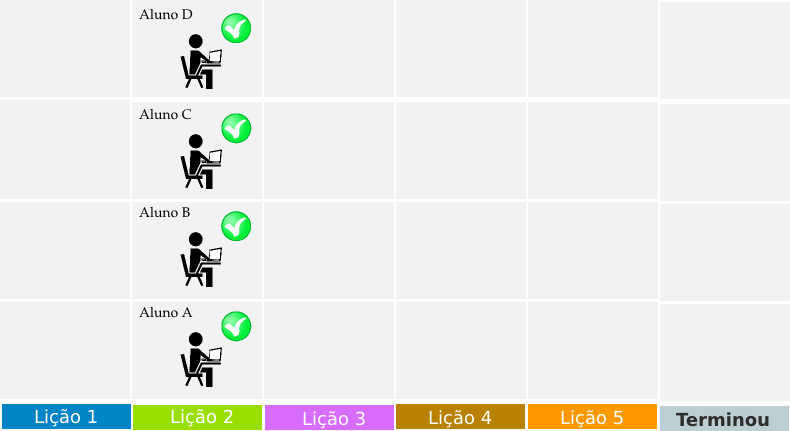
\includegraphics[width=8cm]{figuras/proposta/imagem2.png}
	\floatfoot{Fonte: Elaborada pelo autor}
	\end{figure}
}
\only<+>{
	\begin{figure}[H]
	\centering
	\caption{Representa\c{c}\~ao do nosso Modelo de Aprendizagem}
	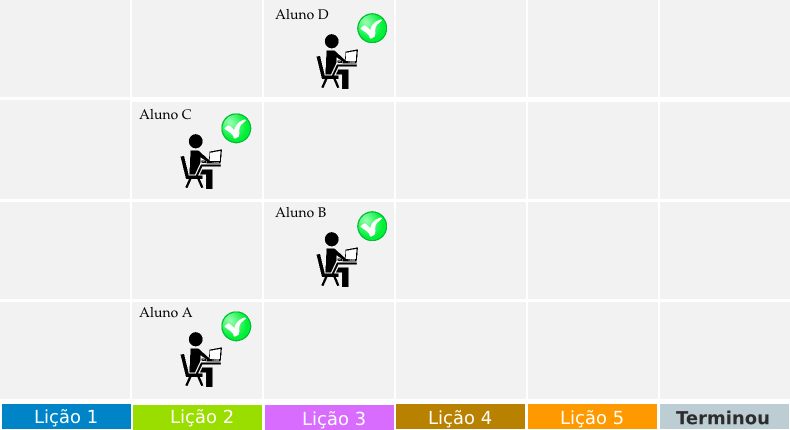
\includegraphics[width=8cm]{figuras/proposta/imagem3.png}
	\floatfoot{Fonte: Elaborada pelo autor}
	\end{figure}
}
\only<+>{
	\begin{figure}[H]
	\centering
	\caption{Representa\c{c}\~ao do nosso Modelo de Aprendizagem}
	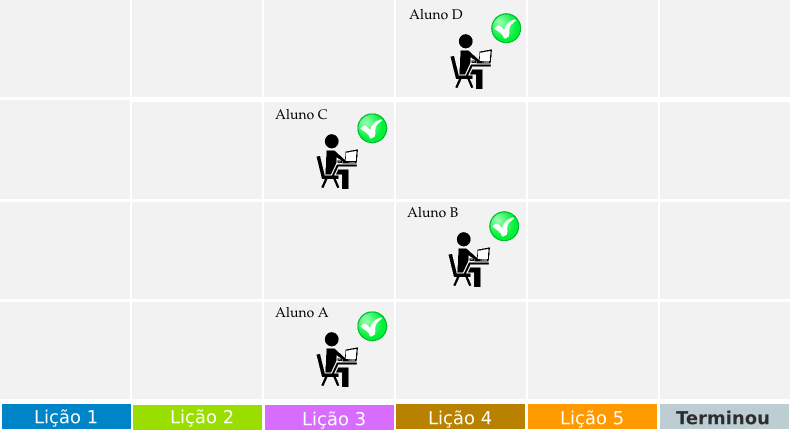
\includegraphics[width=8cm]{figuras/proposta/imagem4.png}
	\floatfoot{Fonte: Elaborada pelo autor}
	\end{figure}
}
\only<+>{
	\begin{figure}[H]
	\centering
	\caption{Representa\c{c}\~ao do nosso Modelo de Aprendizagem}
	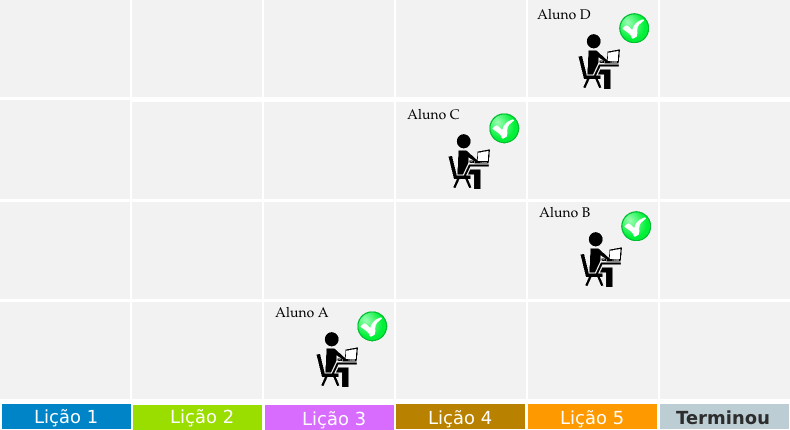
\includegraphics[width=8cm]{figuras/proposta/imagem5.png}
	\floatfoot{Fonte: Elaborada pelo autor}
	\end{figure}
}
\only<+>{
	\begin{figure}[H]
	\centering
	\caption{Representa\c{c}\~ao do nosso Modelo de Aprendizagem}
	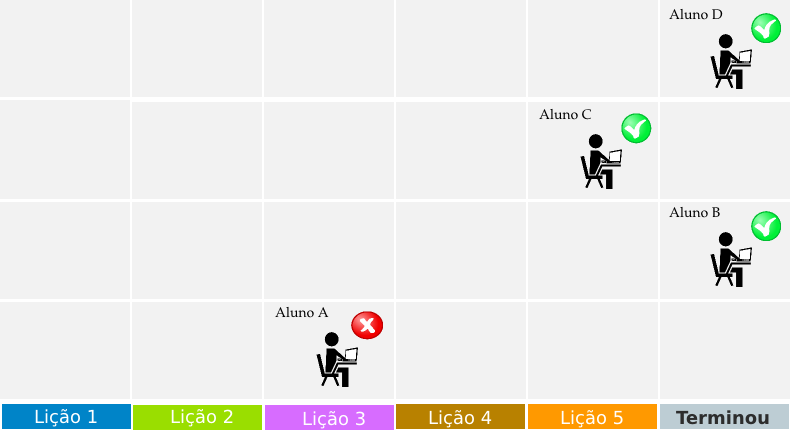
\includegraphics[width=8cm]{figuras/proposta/imagem6.png}
	\floatfoot{Fonte: Elaborada pelo autor}
	\end{figure}
}
\only<+>{
	\begin{figure}[H]
	\centering
	\caption{Representa\c{c}\~ao do nosso Modelo de Aprendizagem}
	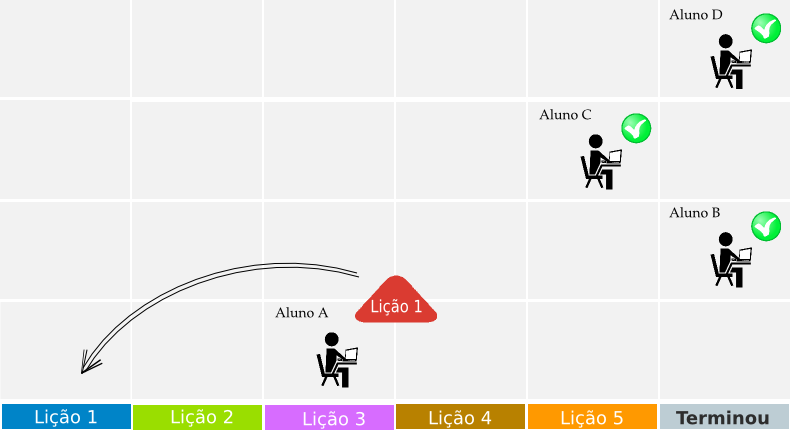
\includegraphics[width=8cm]{figuras/proposta/imagem7.png}
	\floatfoot{Fonte: Elaborada pelo autor}
	\end{figure}
}
\only<+>{
	\begin{figure}[H]
	\centering
	\caption{Representa\c{c}\~ao do nosso Modelo de Aprendizagem}
	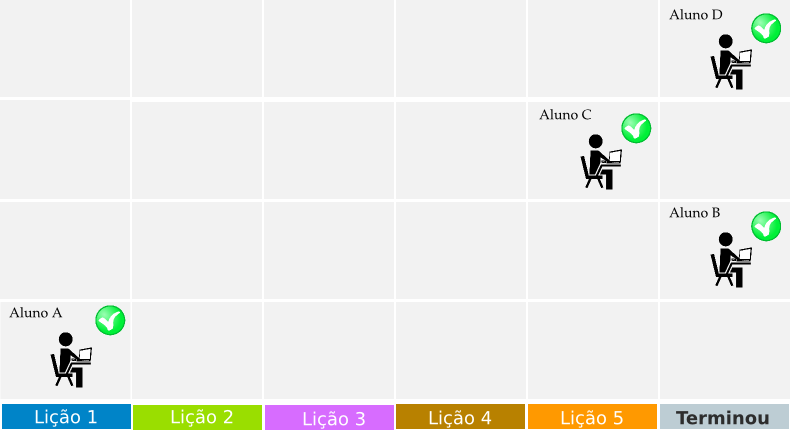
\includegraphics[width=8cm]{figuras/proposta/imagem8.png}
	\floatfoot{Fonte: Elaborada pelo autor}
	\end{figure}
}
\only<+>{
	\begin{figure}[H]
	\centering
	\caption{Representa\c{c}\~ao do nosso Modelo de Aprendizagem}
	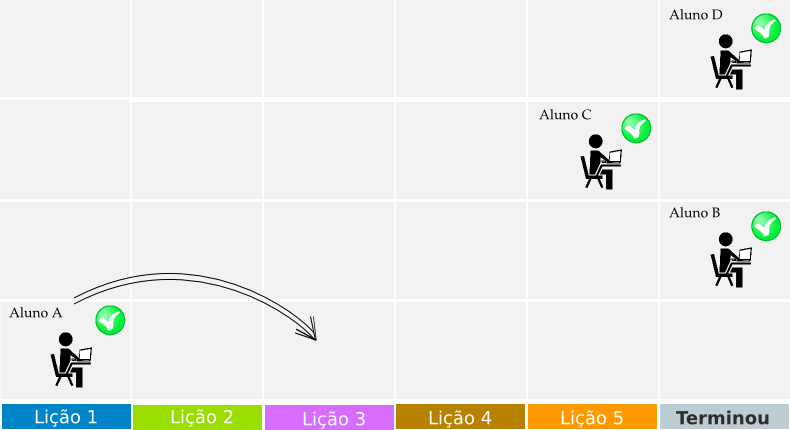
\includegraphics[width=8cm]{figuras/proposta/imagem9.png}
	\floatfoot{Fonte: Elaborada pelo autor}
	\end{figure}
}
\only<+>{
	\begin{figure}[H]
	\centering
	\caption{Representa\c{c}\~ao do nosso Modelo de Aprendizagem}
	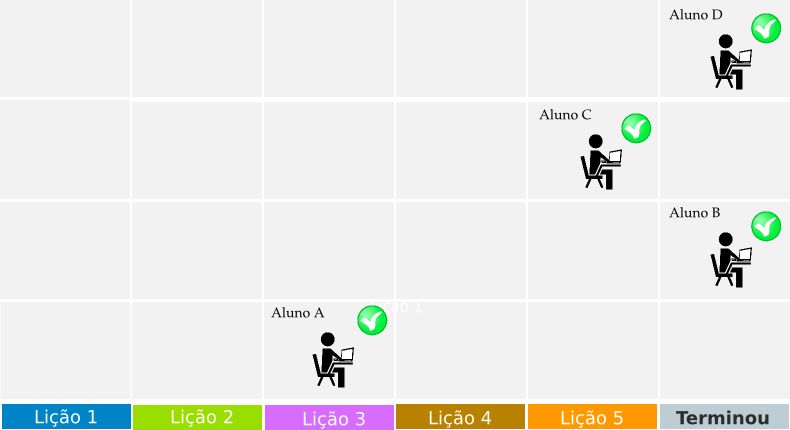
\includegraphics[width=8cm]{figuras/proposta/imagem10.png}
	\floatfoot{Fonte: Elaborada pelo autor}
	\end{figure}
}

\only<+>{
	\begin{figure}[H]
	\centering
	\caption{Representa\c{c}\~ao do nosso Modelo de Aprendizagem}
	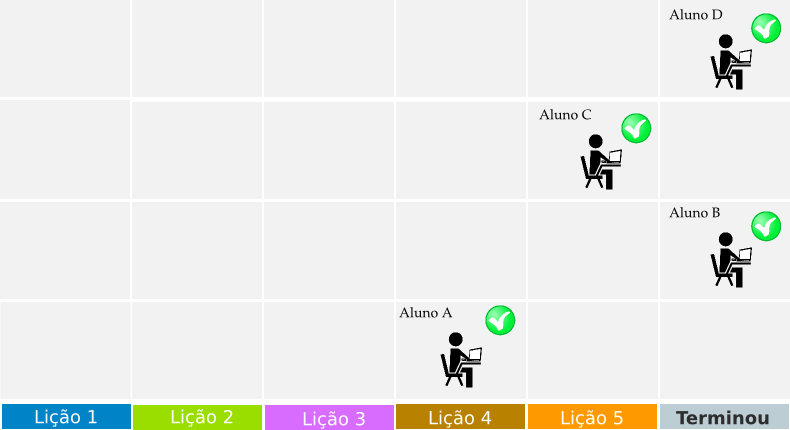
\includegraphics[width=8cm]{figuras/proposta/imagem11.png}
	\floatfoot{Fonte: Elaborada pelo autor}
	\end{figure}
}

\only<+>{
	\setcounter{figure}{4}
	\begin{figure}[H]
	\centering
	\caption{Estrutura do Problema}
	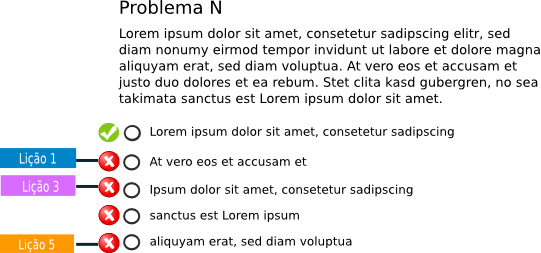
\includegraphics[width=8cm]{figuras/estrutura_problema.png}
	\floatfoot{Fonte: Elaborada pelo autor}
	\end{figure}
}

\only<+>{
	\begin{table}[H]
		\caption{Compara\c{c}\~ao entre os tradicionais modelos de aprendizagem e o nosso.}
		\resizebox{8cm}{!}{
			
			\begin{tabular}{|l|l|}
			\hline
			\textbf{Modelos Tradicionais}                                        & \textbf{Nosso Modelo}                                     
            \\ \hline
			\begin{tabular}[c]{@{}l@{}}Centrado no professor\end{tabular}      & Centrado no aluno                                           
          \\ \hline
			\begin{tabular}[c]{@{}l@{}}Absorção passiva\end{tabular}           & \begin{tabular}[c]{@{}l@{}}Participação ativa do 
aluno\end{tabular} \\ \hline
			O professor como especialista                                        & O professor como guia                                     
            \\ \hline
			Estático                                                             & Dinâmico                                                  
            \\ \hline
			\begin{tabular}[c]{@{}l@{}}Aprendizado predeterminado\end{tabular} & \begin{tabular}[c]{@{}l@{}}Aprender a aprender\end{tabular} 
        \\ \hline
			\end{tabular}
		
		}
		\floatfoot{Fonte: Elaborada pelo autor}
	\end{table}
}


\end{overprint}

\end{frame}

\section{Ferramentas}

% ----------------- NOVO SLIDE --------------------------------
\begin{frame}{Ferramentas utilizadas}

\begin{itemize}
	\item \textbf{Linguagem de Programa\c{c}\~ao}: Python
	\item \textbf{Framework Back-end}: Django
	\item \textbf{Framework Front-end}: Metro UI CSS
	\item \textbf{Plugin de Internacionaliza\c{c}\~ao}: Rosetta
	\item \textbf{Banco de Dados}: PostgreSQL
	\item \textbf{Engine para Latex}: MathJax
\end{itemize}

\end{frame}

\section{Trabalhos Futuros}

% ----------------- NOVO SLIDE --------------------------------
\begin{frame}{Trabalhos Futuros}

\begin{itemize}
	\item Bate-papo entre alunos
	\item 
	\item Vers\~ao para Dispositivos M\'oveis
\end{itemize}

\end{frame}

\section{Refer\^encias}
% ----------------- NOVO SLIDE --------------------------------
\begin{frame}[allowframebreaks]{Refer\^encias}
  \bibliography{demo}
\end{frame}

% ----------------- NOVO SLIDE --------------------------------
\begin{frame}{Coment\'arios}
	\begin{columns}
		\begin{column}{3cm}
			
\includegraphics[height=3cm]{figuras/askmath.png}
		\end{column}
		\begin{column}{7cm}
			\begin{flushright}
				\centering
				\vskip 0.5cm
				\Huge Obrigado!
			\end{flushright}
		\end{column}
	\end{columns}
\end{frame}



\end{document}
